\documentclass[aspectratio=169]{beamer}

% because we need to claim weird things
\newtheorem{claim}{Claim}
\newtheorem{defn}{Definition}
%\newtheorem{lemma}{Lemma}
\newtheorem{thm}{Theorem}
\newtheorem{vita}{Vit\ae}
\newtheorem{qotd}{Quote of the Day}

\usepackage{algorithm}
\usepackage{algpseudocode}
\usepackage{graphics}
\usepackage{ulem}
\bibliographystyle{unsrt}

% background image
\usebackgroundtemplate%
{%
    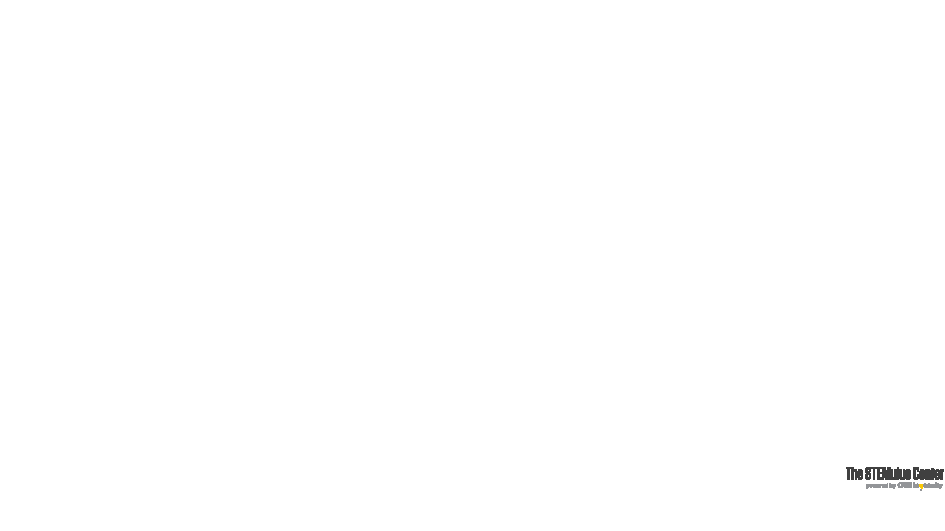
\includegraphics[width=\paperwidth,height=\paperheight]{../artifacts/stemulus.pdf}%
}
\setbeamertemplate{caption}[numbered]

% page numbers
\addtobeamertemplate{navigation symbols}{}{%
    \usebeamerfont{footline}%
    \usebeamercolor[fg]{footline}%
    \hspace{1em}%
    \insertframenumber/\inserttotalframenumber
}

% presentation header
\usetheme{warsaw}
\title{Week 1: Data Design}
\author{Dylan Lane McDonald}
\institute{CNM STEMulus Center\\Web Development with PHP}
\date{\today}

\begin{document}
\begin{frame}
\titlepage
\end{frame}

\begin{frame}
\frametitle{Outline}
\tableofcontents
\end{frame}

\section{Data Modeling}
\begin{frame}
\frametitle{Data Modeling Process}
\begin{itemize}
	\item The Data Modeling Process is used to define and analyze data requirements needed to support the understanding of the data within a problem domain or business context.
	\item The process of data modeling involves data modelers or business analysts working closely with business stakeholders, as well as potential users of the system.
	\item Many believe that data modeling is the process of learning about the data, and the data model is the end result of the data modeling process.
	\item A well engineered information system will typically use three different types of data models while progressing from requirements to the actual database to be used for the information system.
	\item The data requirements are initially recorded as a conceptual data model which is essentially a set of coarse grained data definitions and is used to discuss initial requirements with the business stakeholders. 
%	\item The conceptual model is then translated into a logical data model, which documents in more detail,structures of the data that can be implemented in databases. 
%	\item The last step in data modeling is transforming the logical data model to a physical data model that organizes the data into tables, and accounts for access, performance and storage details.
%	\item Data modeling defines not just data elements, but also their structures and the relationships between them.
%	\item Data modeling may be performed during various types of projects and in multiple phases of projects.
%	\item Data models are progressive; there is no such thing as the final data model for a business or application.
%	\item Instead a data model should be considered a living document that will change in response to a changing business.
\end{itemize}
\end{frame}

\begin{frame}
\frametitle{Example: Data Modeling Twitter}
\begin{defn}
A \textbf{use case} is an explicit list of steps defining interactions between actors in a system to achieve a \textit{goal} in the system.
\end{defn}
\pause
\mbox{}\\
\textbf{Use Case}: A user posts a tweet by accessing the site, writing the content and clicking ``Tweet''.
\pause
\mbox{}\\
\textbf{Important Data Models}: What is required for a tweet to be stored within our systems?
\begin{itemize}
	\item \textbf{Profile}: Essential data about the user
	\item \textbf{Tweet}: All the tweet messages ever posted on our site
	\item \textbf{Others}: Inevitably, more data requirements will arise as the model grows
\end{itemize}
Notice how the complexity of the data model will grow organically over time as the data model is mapped by the developers and stakeholders.
\end{frame}

\section{Three Models}
\subsection{Conceptual Model}
\begin{frame}
\frametitle{Conceptual Model}
\begin{defn}
A \textbf{conceptual model} is a is a map of concepts and their most basic relationships used for databases. This describes the semantics or meaning of an organization and represents a series of assertions or facts about its nature.
\end{defn}
\pause
\mbox{}\\
\textbf{Example relationships}:
\begin{itemize}
	\item Each \textbf{user} can \textbf{tweet} many times.
	\item Each \textbf{user} can favorite many \textbf{tweets}.
	\item Each \textbf{tweet} can be \textbf{retweeted} many times by many \textbf{users}.
\end{itemize}
Enumerating all such relationships completes the conceptual model. The conceptual model is the first step in organizing the data that will drive the web site.
\end{frame}

\subsection{Logical Model}
\begin{frame}
\frametitle{Logical Model}
\begin{defn}
A \textbf{logical model} is a model that standardizes people, places, things and the rules, relationships and the events between them.
\end{defn}
\pause
\mbox{}\\
Logical models can be thought of as a transitional step from the conceptual model to the physical model. The logical model incorporates all the concepts mapped out in the conceptual model and integrate it into a model that can be directly deployed in any database system. A logical model usually takes the form of Unified Modeling Language (UML) and/or an Entity Relationship Diagram (ERD). An example ERD is depicted in Figure \ref{fig:erd}.
\end{frame}

\begin{frame}
\frametitle{Entity Relationship Diagram Symbols}
\begin{figure}
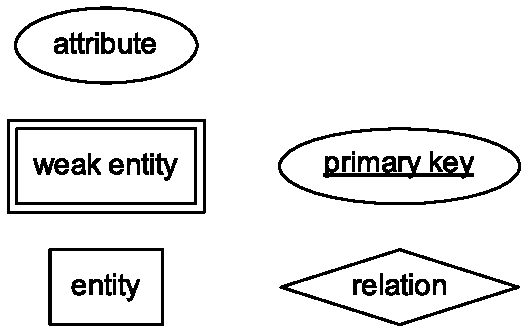
\includegraphics{../artifacts/blank-erd.pdf}
\caption{Entity Relationship Diagram Symbols}
\label{fig:erd}
\end{figure}
\end{frame}

\begin{frame}
\frametitle{Example Entity Relationship Diagram}
\begin{figure}
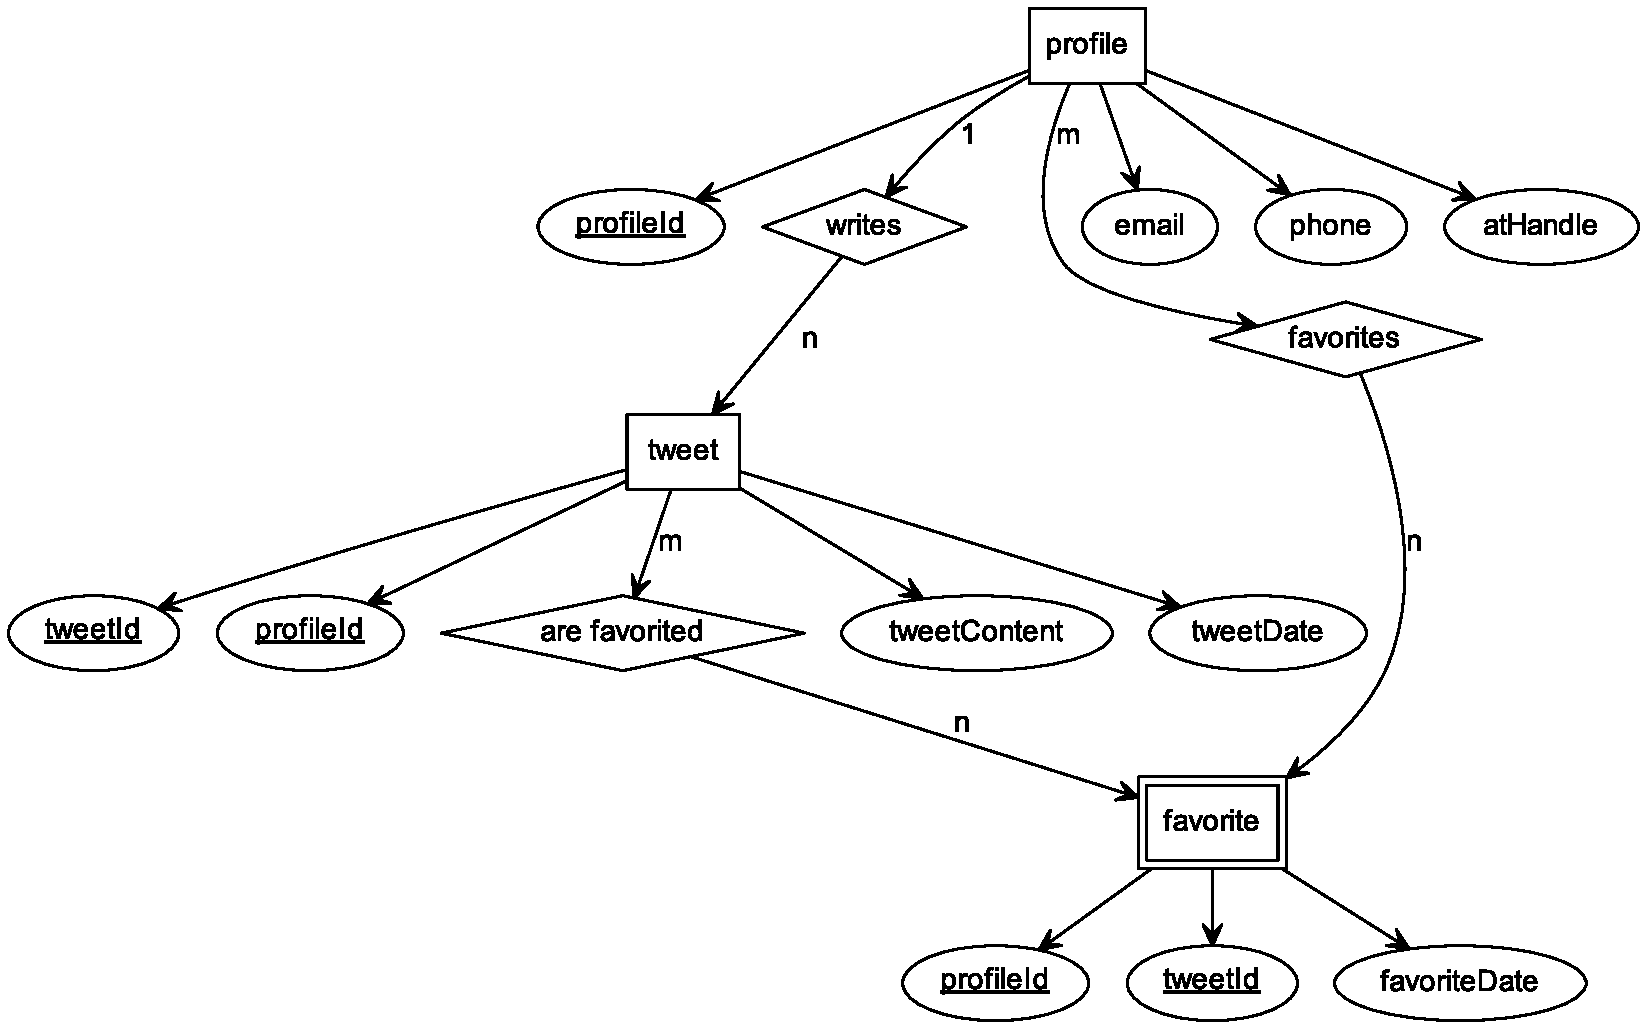
\includegraphics[scale=0.333333333]{../artifacts/twitter-erd.pdf}
\caption{Entity Relationship Diagram for Twitter}
\label{fig:erd}
\end{figure}
\end{frame}

\subsection{Physical Model}
\begin{frame}
\frametitle{Physical Model}
\begin{defn}
A \textbf{physical model} is a series of SQL statements that concretely implements the logical model. A physical model is written for and can be deployed on a specific RDBMS.
\end{defn}
\pause
\mbox{}\\
In mySQL, the physical model will be a \texttt{*.sql} file containing one or more \texttt{CREATE TABLE} statements. The \texttt{CREATE TABLE} statement creates a concrete storage area for data in a mySQL database and describes exactly how the data will be stored and managed.
\end{frame}
\end{document}